\documentclass[10pt]{beamer}
%souza naves, n 576
\usetheme[everytitleformat=regular]{metropolis}

% Língua e acentos
\usepackage[brazil]{babel}
\usepackage[utf8]{inputenc}
\usepackage[T1]{fontenc}

\usepackage{booktabs}
\usepackage[scale=2]{ccicons}

\usepackage{pgfplots}
\usepgfplotslibrary{dateplot}

\title{Fluxo de potência para sistemas de distribuição}
\subtitle{Considerando redução de barras}
\date{\today}
\author{David Maykon Krepsky Silva}
\institute{Departamento de Engenharia Elétrica}
\titlegraphic{\includegraphics[height=1.cm]{img/logo}}

\usepackage{ragged2e}

\usepackage{pgf-pie}
\usetikzlibrary{ shadows }
\usepackage[authoryear]{natbib}

\usepackage{multirow}
\usepackage{subfig}
\usepackage{longtable}

\begin{document}

\maketitle

\begin{frame}
  \frametitle{Sumário}
  \setbeamertemplate{section in toc}[sections numbered]
  \tableofcontents[hideallsubsections]
\end{frame}

\section{Objetivos}
\begin{frame}{Objetivos do trabalho}
    Objetivos primários:
    \begin{itemize}
        \item Implementação dos métodos \textit{Soma de Correntes} e \textit{Soma de potências} para o cálculo do fluxo de potência.
        
        \item Comparação de desempenho entre os métodos.
        
        \item Desenvolvimento e implementação do algoritmo de redução de barras.
    \end{itemize}
    
    Objetivo secundário:
    \begin{itemize}
        \item Desenvolvimento de programa gráfico para análise de sistemas de distribuição utilizando os algoritmos acima citados.
    \end{itemize}
\end{frame}

\section{Metodologia}

\begin{frame}{Metodologia}
    
    \begin{itemize}
        \item Uso de linguagem de programação C++.
        
        \item Desenvolvimento com o \textit{framework} Qt.
        
        \item Validação dos resultados com seis sistemas diferentes.
        
        \item Teste de performance dos algoritmos implementados, com e sem a redução.
    \end{itemize}
\end{frame}

\section{Sistema elétrico brasileiro}

\begin{frame}[fragile]
  \frametitle{Consumo de energia elétrica no Brasil}
    \begin{itemize}
        \item Em julho de 2015, foram consumidos \alert{45.149 GWh} de energia elétrica no Brasil \cite{boletimMME}.
        
        \item As crises hídricas encarecem o custo da energia elétrica, pois estimulam o uso de combustíveis fósseis.
        
        \item De forma a compensar o custo extra das usinas termo-elétricas, foi instaurado em 2015 o Sistema de Bandeiras Tarifárias.
    \end{itemize}
\end{frame}

\begin{frame}[fragile]
    \frametitle{Perfil do consumo - julho/2015}
    \begin{figure}
        \centering
        \caption{Perfil de consumo de energia elétrica no Brasil, julho de 2015}
        \begin{tikzpicture}
            \pie [radius = 2, rotate = 90, color = {green, cyan, orange, black!20, violet, red}, explode = {0, 0, 0, 0, 0, 0.2}, style = drop shadow, text = pin]{22.4/Residêncial, 31.1/Industrial, 15.0/Comercial, 4.5/Rural, 8.4/Outros, 18.5/Perdas}    
        \end{tikzpicture}
        \\
        \small Fonte: Ministério de Minas e Energia \cite{boletimMME}.
        \label{fig:perfil}
        \end{figure}
\end{frame}

\begin{frame}[fragile]
  \frametitle{Ineficiência do sistema}
  \begin{itemize}
      \item Em alguns estados, como no Piauí, as perdas chegam a \alert{29\%} \cite{CostaNorte}.
      
      \item As perdas técnicas (como as perdas nos cabos e nos transformadores) chegam a 13\% \cite{CostaNorte}, sendo maior que as perdas totais em países como os EUA, a qual fica em torno de 6\% \cite{Queiroz}.
      
      \item O prejuízo é avaliado em bilhões de reais por ano.
      
      \item As maiores perdas técnicas se encontram no sistema de distribuição.
    \end{itemize}
\end{frame}

\begin{frame}[fragile]
  \frametitle{Perdas em outros países}
  \begin{figure}
    \centering
    \caption{Perdas elétricas de transmissão e distribuição em \%}
    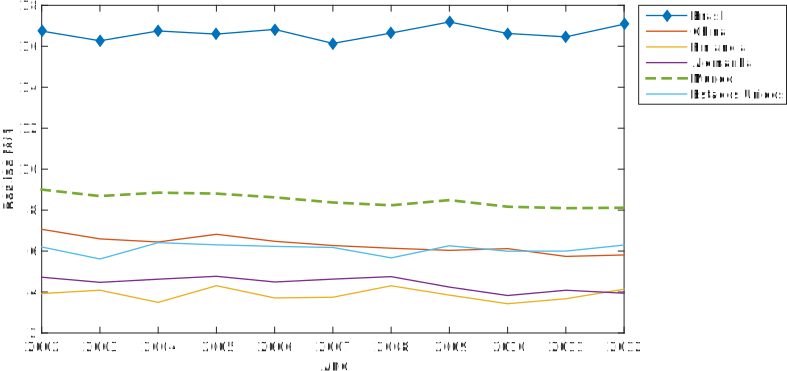
\includegraphics[width=\textwidth]{img/perdas_mundo}
    \\
    \small Fonte: Autoria própria (dados de \textit{World Development Indicators, 2015}).
    \label{fig:mundo}
  \end{figure}
\end{frame}

\section{O fluxo de potência}

\begin{frame}[fragile]
  \frametitle{O que é}
  \justify
     O fluxo de potência (ou fluxo de carga) é um problema matemático, composto por um conjunto de equações algébricas não lineares, que permite determinar os valores de tensão e potência, bem como as perdas, para um sistema elétrico de potência em regime permanente.

\end{frame}

\begin{frame}{Utilidade}
    \justify
    Provê uma visão detalhada das condições de operação do sistema, permitindo:
    
    \begin{itemize}
        \item análise de segurança da rede;
        
        \item o planejamento de redes de transmissão/distribuição mais eficientes;
        
        \item otimização dos sistemas em operação.
       \end{itemize}
\end{frame}

\begin{frame}{Características dos sistemas de potência}
    \begin{itemize}
        \item Composto por \emph{barras}, geradores, cargas, transformadores, reatores \textit{shunt}, capacitores \textit{shunt} e linhas de transmissão/distribuição.
        
        \item Barras são do tipo PV, PQ e V$\theta$.
        
        \item Barras são interligadas por linhas, as quais possuem perdas.
    \end{itemize}
\end{frame}

\begin{frame}{Solução do fluxo de potência}
    \justify
    Devido a natureza não linear do problema, são necessários métodos numéricos iterativos para a determinar uma aproximação das incógnitas nas equações do fluxo de potência.
\end{frame}


\begin{frame}{Métodos para cálculo do fluxo de potência}
    \justify
    Apesar dos métodos de Gauss-Seidel e Newton-Raphson (e seus derivados) serem amplamente utilizados para o calculo do fluxo de potência em sistemas de transmissão de energia elétrica, os mesmos apresentam problemas de convergência e desempenho quando aplicados em sistemas de distribuição \cite{Eminoglu, Alsaadi, Reddy, Yao}.
\end{frame}

\section{Métodos para redes de distribuição}

\begin{frame}{Redes de distribuição}
    Os métodos empregados na solução de redes de distribuição aproveitam a topologia radial \cite{Cespedes}, ou fracamente malhada \cite{ShirmohammadiMono, Shirmohammadi3F}, para resolver o problema do fluxo de potência.
\end{frame}

\begin{frame}{Redes radiais}
\begin{figure}[H]
   \centering
   \caption{Sistema radial.}
   \includegraphics[scale=0.2]{img/70b}
   \label{fig:70b}
\end{figure}
\end{frame}

\begin{frame}{Redes malhadas}
    \begin{figure}[H]
        \centering
        \caption{Sistema malhado.}
        \includegraphics[scale=0.6]{img/malhado}
        \label{fig:malhado}
    \end{figure}
\end{frame}

\begin{frame}{Método Soma de Potências (MSP)}
    Este método, proposto em \citep{Cespedes}, consiste em duas operações, uma a montante e outra a jusante. 
    
    \begin{itemize}
        \item Operação a montante: partindo dos nós finais até o nó inicial, são calculadas as potências equivalentes em cada nó (i.e., somando todas as potências que são alimentadas por cada nó e as suas perdas).
        
        \item Operação a jusante: dado que a tensão da barra de referência é conhecida, é aplicada a equação \ref{equ:cespedes} para o cálculo da tensão nas barras subsequentes.
        
        \item O critério de parada é determinado pela variação das perdas totais do sistema (equação \ref{equ:cespedesL}).
    \end{itemize}
\end{frame}

\begin{frame}{Método Soma de Potências}
    Equação para o cálculo das tensões:
    \begin{equation}
      \label{equ:vcespedes2}
      |V_j|^4 + [2 \cdot (PR+QX) -  |V_i|^2] \cdot  |V_j|^2 + (P^2 + Q^2) \cdot (R^2 + X^2) = 0.  
    \end{equation}
  
  onde:
  \begin{itemize}
    \item \emph{i}: nó fonte;
    \item \emph{j}: nó à jusante;
    \item \emph{$V_i$}: módulo da tensão em \emph{i};
    \item \emph{$V_j$}: módulo da tensão em \emph{j};
    \item \emph{P}: potência ativa equivalente da carga em \emph{j}; 
    \item \emph{Q}: potência reativa equivalente da carga em \emph{j}; 
    \item \emph{R}: resistência própria da linha;
    \item \emph{X}: reatância própria da linha.
  \end{itemize}

\end{frame}

\begin{frame}{Método Soma de Potências}
    Perdas nas linhas:
    \begin{eqnarray}
    \label{equ:cespedesL}
    L_p = R \frac{(P^2 + Q^2)}{V_j^2} \\
    L_q = X \frac{(P^2 + Q^2)}{V_j^2}
    \end{eqnarray}
\end{frame}

\begin{frame}{Desvantagens}
Desvantagens:
    \begin{itemize}
        \item aplicável somente a sistemas radiais;
        \item não considera o acoplamento entre linhas.
    \end{itemize}
\end{frame}

\begin{frame}{Método Soma de Correntes (MSC)}
    Proposto em \cite{ShirmohammadiMono, Shirmohammadi3F}, também consiste em duas operações, chamadas de varredura para trás (\textit{backward sweep}) e varredura para frente (\textit{forward sweep}). 
    
    \begin{itemize}
        \item Varredura para trás: assumindo um perfil de tensão inicial para as barras, o algoritmo começa calculando as correntes nos nós das camadas finais com a equação \ref{equ:shirmI}. Em seguida, é calculado a corrente da camada anterior, sendo que, a corrente nas barras dessa camada é a soma das correntes que vão e direção a camada seguinte (equação \ref{equ:shirmJ}).
        
        \item Varredura para frente: Ao chegar na barra de referência (a qual possui tensão e fase conhecidas), o algoritmo calcula a tensão nas barras subsequentes, considerando as correntes previamente calculadas e a queda de tensão nas linhas de distribuição, com a equação \ref{equ:shirmV}.
        
        \item O critério de parada é determinado pela variação da potência no sistema.
    \end{itemize}
\end{frame}

\begin{frame}{Equações do método Soma de Correntes}
   Corrente nas barras:
    \begin{equation}
    \label{equ:shirmI}
      \left[ \begin{matrix}
      I_{ia} \\
      I_{ib} \\
      I_{ic} \\
      \end{matrix} \right]  = 
      \left[ \begin{matrix}
      \left(S_{ia} \big / V_{ia}^{(k-1)} \right)^* \\
      \left(S_{ib} \big / V_{ib}^{(k-1)} \right)^* \\
      \left(S_{ic} \big / V_{ic}^{(k-1)} \right)^* \\
      \end{matrix} \right] -
      \left[ \begin{matrix}
      Y_{ia}^* & & \\
      & Y_{ib}^* & \\
      & & Y_{ic}^* \\
      \end{matrix} \right]
      \left[ \begin{matrix}
      V_{ia} \\
      V_{ib} \\
      V_{ic} \\
      \end{matrix} \right]^{(k-1)}
    \end{equation}
 
    Corrente nas linhas:
    \begin{equation}
    \label{equ:shirmJ}
     \left[ \begin{matrix}
     J_{la} \\
     J_{lb} \\
     J_{lc} \\
     \end{matrix} \right]^{(k)}  = -
      \left[ \begin{matrix}
      I_{ja} \\
      I_{jb} \\
      I_{jc} \\
      \end{matrix} \right]^{(k)} + \sum_{m \, \in \, M}
       \left[ \begin{matrix}
       J_{ma} \\
       J_{mb} \\
       J_{mc} \\
       \end{matrix} \right]^{k}
    \end{equation}
    
        Tensão nas barras:
        \begin{equation}
        \label{equ:shirmV}
        \left[ \begin{matrix}
        V_{ja} \\
        V_{jb} \\
        V_{jc} \\
        \end{matrix} \right]^{(k)}  =
        \left[ \begin{matrix}
        V_{ia} \\
        V_{ib} \\
        V_{ic} \\
        \end{matrix} \right]^{(k)} -
        \left[ \begin{matrix}
        Z_{aa,l} & Z_{ab,l} &  Z_{ac,l} \\
        Z_{ba,l} & Z_{bb,l} &  Z_{bc,l} \\
        Z_{ca,l} & Z_{cb,l} &  Z_{cc,l} \\
        \end{matrix} \right]
        \left[ \begin{matrix}
        J_{la} \\
        J_{lb} \\
        J_{lc} \\
        \end{matrix} \right]^{(k)}
        \end{equation}
\end{frame}

\begin{frame}{Equações do método Soma de Correntes}
 Onde:
 
    \begin{itemize}
    \item $I_{ia}, I_{ib}, I_{ic}$ são as injeções de corrente na barra \emph{i}.
    
    \item $S_{ia}, S_{ib}, S_{ic}$ são as injeções de potência programadas na barra \emph{i}.
    
    \item $V_{ia}, V_{ib}, V_{ic}$ são as tensões na barra \emph{i}.
    
    \item $Y_{ia}, Y_{ib}, Y_{ic}$ são as admitâncias dos elementos \textit{shunt} na barra \emph{i}.
    
    \item $J_{la}, J_{lb}, J_{lc}$ são as correntes na linha \emph{l}.
    
    \item \emph{k} é a iteração.
    \end{itemize}
    
    
\end{frame}

\begin{frame}{Algoritmo de redução de barras}
    Parte do princípio de que barras inertes podem ser removidas do sistema sem causar divergência no fluxo de potência.
\end{frame}

\begin{frame}{Algoritmo de redução de barras}
    \begin{figure}[h]
      \centering
      \caption{Sistema radial monofásico com 6 barras.}
      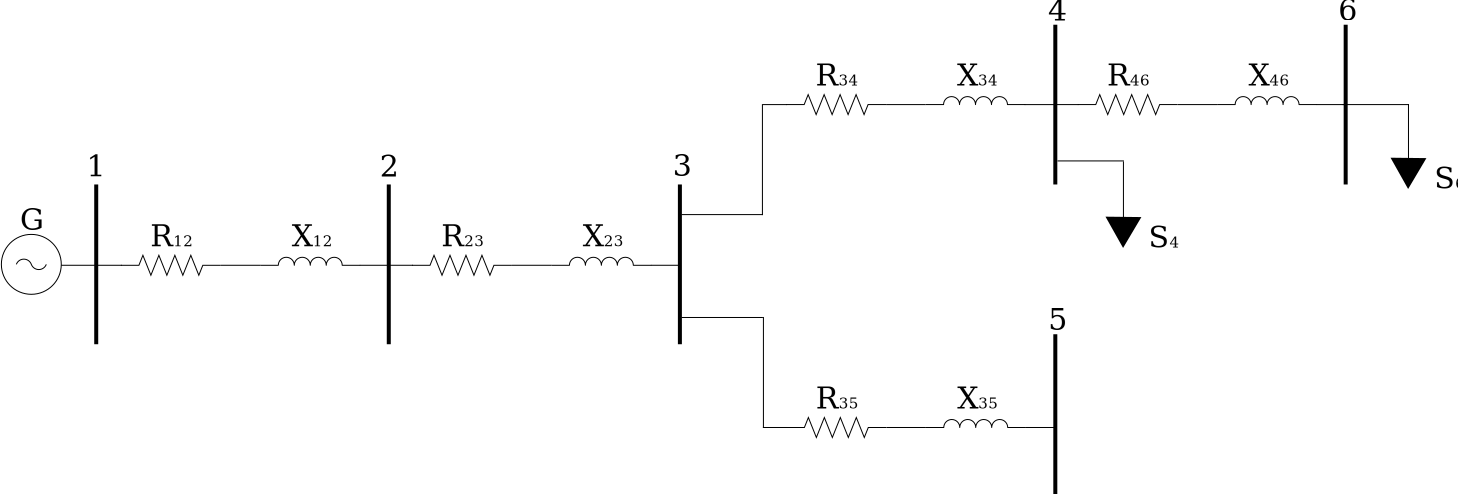
\includegraphics[width=\textwidth]{img/barreduc}
      \label{fig:barreduc}
      
      \small Fonte: Autoria própria.
    \end{figure}
\end{frame}

\begin{frame}{Algoritmo de redução de barras}
 \begin{figure}[h]
   \centering
   \caption{Conexão entre as barras 3 e 5 para o sistema da figura \ref{fig:barreduc}.}
   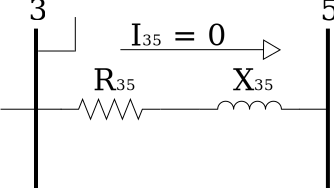
\includegraphics[scale=0.7]{img/barreduc1}
   \label{fig:barreduc1}
   
   \small Fonte: Autoria própria.
  \end{figure}
\end{frame}

\begin{frame}{Algoritmo de redução de barras}
    \begin{figure}[h]
      \centering
      \caption{Conexão entre as barras \textit{1} e \textit{3} da figura \ref{fig:barreduc}.}
      \label{fig:barreduc2}
      
      \subfloat[Com a barra 2.]{%
        \label{fig:barreduc2a}
        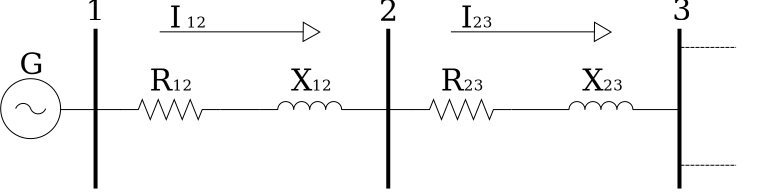
\includegraphics[scale=0.35]{img/barreduc2}
      }
      
      \subfloat[Sem a barra 2.]{%
        \label{fig:barreduc2b}
        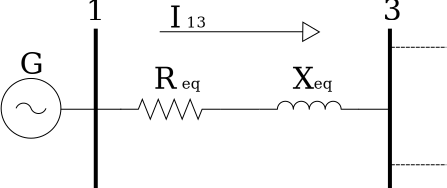
\includegraphics[scale=0.35]{img/barreduc3}
      }
      
      \small Fonte: Autoria própria.
    \end{figure}
\end{frame}

\begin{frame}{Algoritmo de redução de barras}
  \begin{figure}[h]
    \centering
    \caption{Sistema reduzido.}
    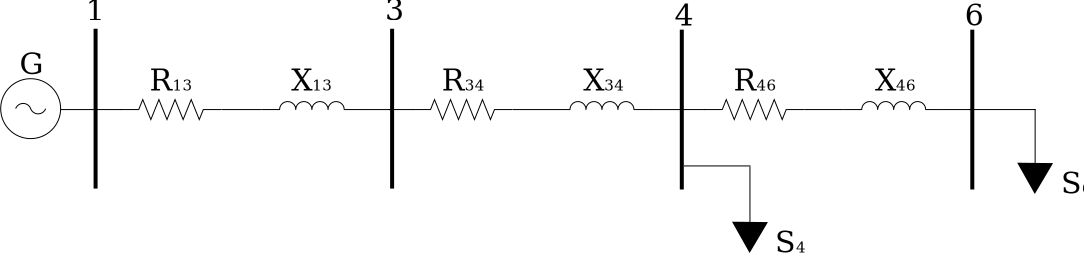
\includegraphics[width=\textwidth]{img/barreduc4}
    \label{fig:barreduc4}
    
    \small Fonte: Autoria própria.
  \end{figure}
\end{frame}

\begin{frame}{Comparação entre os algoritmos - Tensão monofásica}
  Reinsere as barras removidas no sistema, calculando sua tensão.
  
  Para sistemas monofásicos, não há divergência nos resultados.
  
  Para sistemas trifásicos, há uma variação nos valores das barras reinseridas.
  
\end{frame}
\section{Resultados}

\begin{frame}{Comparação entre os algoritmos - Tensão monofásica}
    \begin{longtable}{lllr}
      \caption{Módulo da tensão de linha nas barras do sistema de 14 barras.}\label{tab:14b_v}\\
      \toprule
      \multirow{2}{*}{\textbf{Barra}}& \multicolumn{2}{c}{\textbf{Tensão [V]}}&\multirow{2}{*}{\textbf{$\mathbf{\Delta}$V [\%]}}\\
      & \multicolumn{1}{c}{MSC} & \multicolumn{1}{c}{MSP} & \\
      \midrule
      \endfirsthead
      
      \multicolumn{4}{c}%
      {{\bfseries \tablename\ \thetable{} -- continuação da página anterior}} \\
      \toprule
      \multirow{2}{*}{\textbf{Barra}}& \multicolumn{2}{c}{\textbf{Tensão [V]}}&\multirow{2}{*}{\textbf{$\mathbf{\Delta}$V [\%]}}\\
      & \multicolumn{1}{c}{MSC} & \multicolumn{1}{c}{MSP} & \\
      \midrule
      \endhead
      
      \midrule \multicolumn{4}{r}{{Continua na próxima página}} \\
      \endfoot
      
      \bottomrule \multicolumn{4}{c}{\small Fonte: Autoria própria.}
      \endlastfoot
      
      0&13279.0562&13279.0562&0\\
      3&13155.1064&13155.1064&0\\
      4&13116.8665&13116.8665&0\\
      5&13093.0194&13093.0194&0\\
      6&13078.4579&13078.4579&0\\
      7&13000.9878&13000.9878&0\\
      8&12894.9325&12894.9325&0\\
      9&12972.5789&12972.5789&0\\
      10&12893.4175&12893.4175&0\\
      11&12870.9415&12870.9415&0\\

    \end{longtable}
    
\end{frame}

\begin{frame}{Validação dos algoritmos - Perdas monofásicas}
\begin{longtable}{llllr}
  \caption{Comparação entre as perdas nas linhas do sistema de 14 barras.}\label{tab:14b_l}\\
  \toprule
  \multirow{2}{*}{$\mathbf{Barra_i}$}&\multirow{2}{*}{$\mathbf{Barra_f}$}&\multicolumn{2}{c}{$\mathbf{S_{perda} [kVA]}$}&\multirow{2}{*}{$\mathbf{\Delta S_{perda} [kVA]}$}\\
  && \multicolumn{1}{c}{MSC} & \multicolumn{1}{c}{MSP} & \\
  \midrule
  \endfirsthead
  
  \multicolumn{5}{c}%
  {{\bfseries \tablename\ \thetable{} -- continuação da página anterior}} \\
  \toprule
  \multirow{2}{*}{$\mathbf{Barra_i}$}&\multirow{2}{*}{$\mathbf{Barra_f}$}&\multicolumn{2}{c}{$\mathbf{S_{perda} [kVA]}$}&\multirow{2}{*}{$\mathbf{\Delta}S_{perda} [\%]$}\\
  && \multicolumn{1}{c}{MSC} & \multicolumn{1}{c}{MSP} & \\
  \midrule
  \endhead
  
  \midrule \multicolumn{5}{r}{{Continua na próxima página}} \\
  \endfoot
  
  \bottomrule \multicolumn{5}{c}{\small Fonte: Autoria própria.}
  \endlastfoot
  
  0&3&61.63 + 82.17i&61.63 + 82.17i&0\\
  0&7&278.33 + 278.33i&278.33 + 278.33i&0\\
  0&12&29.07 + 29.07i&29.07 + 29.07i&0\\
  3&4&7.51 + 10.32i&7.51 + 10.32i&0\\
  3&5&11.94 + 23.89i&11.94 + 23.89i&0\\
  5&6&1.52 + 1.52i&1.52 + 1.52i&0\\
  7&8&87.01 + 119.63i&87.01 + 119.63i&0\\
  7&9&2.08 + 2.080i&2.08 + 2.08i&0\\
  8&10&0.71 + 0.710i&0.71 + 0.710i&0\\

\end{longtable}
\end{frame}

\begin{frame}{Comparação entre os algoritmos - Tensão trifásica}
  \begin{longtable}{lllr}
    \caption{Módulo da tensão de linha nas barras do sistema de 34 barras (fase $a$).}\label{tab:34b_va}\\
    \toprule
    \multirow{2}{*}{\textbf{Barra}}& \multicolumn{2}{c}{\textbf{Tensão [V]}}&\multirow{2}{*}{\textbf{$\mathbf{\Delta}$V [\%]}}\\
    & \multicolumn{1}{c}{MSC} & \multicolumn{1}{c}{MSP} & \\
    \midrule
    \endfirsthead
    
    \multicolumn{4}{c}%
    {{\bfseries \tablename\ \thetable{} -- continuação da página anterior}} \\
    \toprule
    \multirow{2}{*}{\textbf{Barra}}& \multicolumn{2}{c}{\textbf{Tensão [V]}}&\multirow{2}{*}{\textbf{$\mathbf{\Delta}$V [\%]}}\\
    & \multicolumn{1}{c}{MSC} & \multicolumn{1}{c}{MSP} & \\
    \midrule
    \endhead
    
    \midrule \multicolumn{4}{r}{{Continua na próxima página}} \\
    \endfoot
    
    \bottomrule \multicolumn{4}{c}{\small Fonte: Autoria própria.}
    \endlastfoot
    
    0&14376.0217&14376.0217&0\\
    2&14328.2494&14317.0068&-0.078465\\
    6&14296.1153&14277.4644&-0.13046\\
    8&13696.3155&13545.2221&-1.1032\\
    10&13696.3155&13545.2221&-1.1032\\
    12&13004.399&12705.208&-2.3007\\
    56&12093.691&11579.1058&-4.255\\
    64&11671.7313&11048.7036&-5.3379\\
    88&11698.3139&11080.3959&-5.2821\\
    90&11658.4819&11025.2575&-5.4314\\
  \end{longtable}
\end{frame}

\begin{frame}{Validação dos algoritmos - Perdas trifásicas}
\begin{longtable}{lllr}
  \caption{Módulo da tensão de linha nas barras do sistema de 34 barras (fase $b$).}\label{tab:34b_vb}\\
  \toprule
  \multirow{2}{*}{\textbf{Barra}}& \multicolumn{2}{c}{\textbf{Tensão [V]}}&\multirow{2}{*}{\textbf{$\mathbf{\Delta}$V [\%]}}\\
  & \multicolumn{1}{c}{MSC} & \multicolumn{1}{c}{MSP} & \\
  \midrule
  \endfirsthead
  
  \multicolumn{4}{c}%
  {{\bfseries \tablename\ \thetable{} -- continuação da página anterior}} \\
  \toprule
  \multirow{2}{*}{\textbf{Barra}}& \multicolumn{2}{c}{\textbf{Tensão [V]}}&\multirow{2}{*}{\textbf{$\mathbf{\Delta}$V [\%]}}\\
  & \multicolumn{1}{c}{MSC} & \multicolumn{1}{c}{MSP} & \\
  \midrule
  \endhead
  
  \midrule \multicolumn{4}{r}{{Continua na próxima página}} \\
  \endfoot
  
  \bottomrule \multicolumn{4}{c}{\small Fonte: Autoria própria.}
  \endlastfoot
  
  0&14376.0217&14376.0217&0\\
  2&14335.786&14320.2529&-0.10835\\
  6&14309.7979&14283.7781&-0.18183\\
  8&13844.7644&13624.9811&-1.5875\\
  64&11873.0989&11106.6181&-6.4556\\
  88&11918.0186&11151.7078&-6.4299\\
  90&11882.2571&11096.926&-6.6093\\
\end{longtable}
\end{frame}

\begin{frame}{Comparação de desempenho - Tempo}
  \begin{figure}[h!]
    \centering
    \caption{Tempo de execução dos algoritmos do fluxo de potência.}
    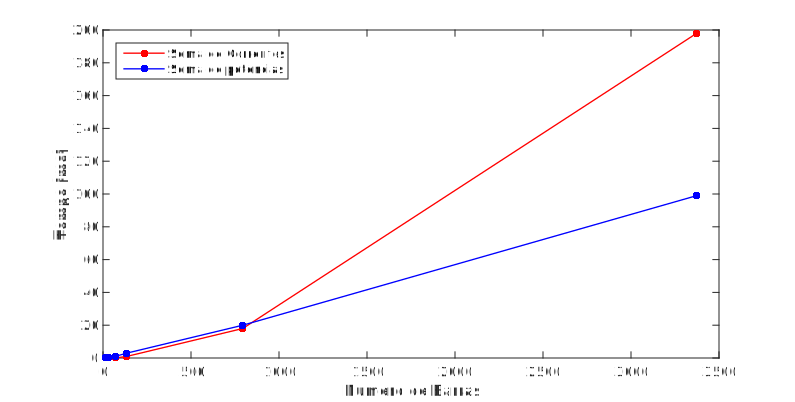
\includegraphics[scale=0.5]{img/tempo}
    \label{fig:tempo}
    
    \small Fonte: Autoria própria.
  \end{figure}
\end{frame}

\begin{frame}{Comparação de desempenho - Iterações}
  \begin{figure}[h!]
    \centering
    \caption{Número de iterações necessárias para convergência dos sistemas de teste.}
    \includegraphics[scale=0.5]{img/itera}
    \label{fig:itera}
    
    \small Fonte: Autoria própria.
  \end{figure}
\end{frame}

\begin{frame}{Sistemas reduzidos}
    \begin{table}[h]
      \centering
      \caption{Barras removidas.}
      \begin{tabular}{cccc}
        \toprule
        \multicolumn{1}{c}{\textbf{Sistema original}} & \textbf{Barras} & \multicolumn{1}{c}{\textbf{Sistema reduzido}} & \multirow{ 2}{*}{\textbf{Redução [\%]}} \\
        \multicolumn{1}{c}{\textbf{[barras]}}& \textbf{removidas} & \multicolumn{1}{c}{\textbf{[barras]}} & \\
        \midrule
        14		& 0    & 14  & 0 \\
        34		& 5    & 29  & 14,7 \\
        70		& 18   & 52  & 25,7 \\
        136		& 24   & 112 & 17,6 \\
        793		& 428  & 365 & 54,0 \\
        3373  & 2748 & 625 & 81,5 \\
        \bottomrule
      \end{tabular}
      \label{tab:tempootm}
      
      \small Fonte: Autoria própria.
    \end{table}
\end{frame}

\begin{frame}{Comparação de desempenho com redução - Tempo}
  \begin{figure}[h!]
    \centering
    \caption{Tempo de execução dos algoritmos do fluxo de potência.}
    \includegraphics[scale=0.5]{img/tempootm}
    \label{fig:tempootm}
    
    \small Fonte: Autoria própria.
  \end{figure}
\end{frame}

\begin{frame}{Comparação de desempenho com redução - Iterações}
  \begin{figure}[h!]
    \centering
    \caption{Número de iterações necessárias para convergência dos sistemas de teste.}
    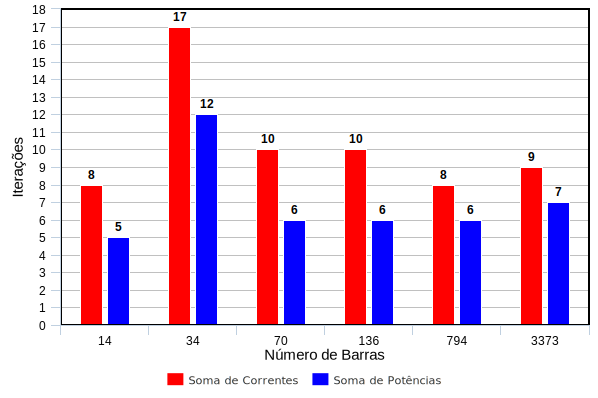
\includegraphics[scale=0.5]{img/iteraotm}
    \label{fig:iteraotm}
    
    \small Fonte: Autoria própria.
  \end{figure}
\end{frame}

\begin{frame}{Erro introduzido pela expansão - Monofásico}
  Não há variação nos resultados para os sistemas monofásicos.
\end{frame}

\begin{frame}{Erro introduzido pela expansão - Trifásico}
  \small
\begin{table}[h]
  \centering
  \caption{Erro devido a expansão do sistema reduzido (34 barras).}
  \begin{tabular}{ccccc}
    \toprule
    \multirow{2}{*}{\textbf{Fase}} & \multirow{2}{*}{$ \mathbf{Erro_{máx}^{MSC}\,[V]} $} & \multirow{2}{*}{$ \mathbf{Erro_{máx}^{MSP}\,[V]} $} & $ \mathbf{Erro_{máx}^{MSC}} $ \textbf{em} & $ \mathbf{Erro_{máx}^{MSP}} $ \textbf{em}\\
    &&& \textbf{relação a} $\mathbf{V_{base}}$ \textbf{[\%]}& \textbf{relação a} $\mathbf{V_{base}}$ \textbf{[\%]}\\
    \midrule
    $a$		& 127 & 362  & 0,88 & 2,52 \\
    $b$		& 235 & 2760 & 1,63 & 19,19 \\
    $c$		& 56  & 1.090& 0.39 & 7,58 \\
    \bottomrule
  \end{tabular}
  \label{tab:erro}
  
  \small Fonte: Autoria própria.
\end{table}
\normalsize
\end{frame}

\begin{frame}{\textit{QuickFlow}}
    \begin{figure}[H]
        \centering
        \caption{Programa \textit{QuickFlow} para projeto e análise de sistemas de distribuição de energia elétrica.}
        \includegraphics[scale=0.22]{img/quickflow}
        \label{fig:quickflow}
    \end{figure}
\end{frame}

\begin{frame}{\textit{QuickFlow}}
    \begin{figure}[H]
        \begin{itemize}
            \item Permite a criação, importação e modificação de sistemas de distribuição energia elétrica trifásicos.
            
            \item Possibilita o trabalho com várias unidades (metro, kilometro, pés, milhas e etc.).
             
            \item Permite trabalhar com múltiplos alimentadores.
             
            \item Realiza o cálculo do fluxo de potência utilizando os dois métodos citados anteriormente.
            
            \item Aplica a otimização por redução de barras para agilizar os cálculos (em desenvolvimento).
            
            \item Possui código fonte aberto. Está disponível em \href{http://www.github.com/DKrepsky/QuickFlow}{GitHub/QuickFlow}.
            
        \end{itemize}
    \end{figure}
\end{frame}

\begin{frame}{Conclusão}
    Foi observado que os métodos de resolução do fluxo de potência, empregados no trabalho, se mostram bastante robustos em relação à convergência. O desempenho dos mesmos é satisfatório, sendo necessário poucos milissegundos, em um computador de uso pessoal, para o cálculo dos parâmetros em sistemas compostos por milhares de barras. 
    
    Em relação a comparação entre os métodos, foi possível observar um melhor desempenho do método da soma das potências, porém, o mesmo não o acoplamento entre as linhas, nos sistemas trifásicos.
    
    A redução de barras demonstrou uma melhora considerável no desempenho dos algoritmos do fluxo de potência, porém, em sistemas trifásicos, foi produzido um erro significativo para o método MSP.
    
    Quanto a \textit{interface} gráfica, a mesma se mostrou bastante útil na análise de sistemas de distribuição de energia elétrica, agilizando a avaliação dos resultados e o teste com sistemas diferentes.
\end{frame}

\begin{frame}{Considerações finais}
    O trabalho desenvolvido é um passo inicial no desenvolvimento de uma ferramenta para análise do fluxo de potência. Assim, há a possibilidade de explorar uma grande quantidade de outros algoritmos, tanto de cálculo, como de formas de otimização para o fluxo de potência.
    Uma outra possibilidade é a integração de métodos para o calculo do fluxo de potência ótimo, o qual encontra o melhor estado de operação da rede, de modo a minimizar o custo do kilowatt hora entregue ao consumidor final.
\end{frame}

\begin{frame}[allowframebreaks]

  \frametitle{Referências}

  \bibliography{referencias}
  \bibliographystyle{plain}

\end{frame}

\plain{Muito Obrigado!}

\plain{Perguntas?}

\end{document}
